% !TEX root = ../paper.tex

\section{Case Study}

Our case study used the Qt project review history from the Gerrit code review tool provided by Hamasaki et. al. \cite{Hamasaki2013}. Qt project is a large open source project composed of numerous small subsystems. We selected the most active subproject, which is called \texttt{qtbase}.
From this subproject, we used the review history from May 2011 to June 2012, which contains 6,605 changes and 72,484 comments.


\subsection{Data Preparation}
We used the commit messages and comments in the dataset.
Before classifying the usefulness of comments, we first processed the commit message and comments as follows: 

\subsubsection{Removal of automatically generated messages} To consider only reviewers discussion, we ignored all messages that automatically generated.
%In Gerrit, the comment history is composed of human-written comments from reviewers and automatically generated messages.
These automatic messages are generated by Gerrit, continuous integration system, and the sanity bot\footnote{It is a bot that automatically checks new proposed changes for trivial sanity issues, such as line endings, copyright notices, and commit messages} to record activities. \textit{`Upload patch set 1.'}, \textit{`Change has been successfully cherry-picked to the staging branch as ...'}, and \textit{`Sanity review passed'} are some examples. In practice, they are not considered in code review  and are not substantially relevant to the proposed changes and do not directly impact software quality\cite{Mcintosh}. 

To do so, we first ignore all comments written by bots (i.e. \emph{Qt Continuous Integration System} and \emph{Qt Sanity Bot}). Second, we removed message including reviewers comments by finding common patterns frequently occurred using regular expression. This would leave us only human-written comments that will be used in further preprocessing.

%, . and hence are useless by our definition.
%%They are easily determined as useless by our method and would artificially improve our classification performance.
%These messages are identified by looking for the most common lines of text using regular expression.
%%Regular expression patterns are then constructed to match and remove these messages.
%Occurrences of these patterns are then removed from our dataset prior to further preprocessing.
%
%Automatic messages are also often inserted as part of review comments.
%They too are removed from our dataset, leaving us with only human-written part.
%We also completely ignored comments whose author is \emph{Qt Continuous Integration System} and \emph{Qt Sanity Bot}.

\subsubsection{Data preprocessing}
As is customary for VSM processing, we extracted semantic words from commit messages and comment messages before converting to vector.
For each message, we removed all punctuation signs (except apostrophe) and other non alphanumeric characters. We also removed common words (e.g. a, an, the) using Google stop word list\footnote{Available at \url{http://meta.wikimedia.org/wiki/Stop_word_list/google_stop_word_list#English}}. We then used Porter stemming algorithm to remove the commoner morphological and inflexional endings from words in English.

Table \ref{tb:datastatistic} summarizes data set we used for this study after preparation. 

\begin{table}[!h]
\caption{A summary data sets and some statistics.}
\centering
\small
\begin{tabular}{ccc}
\hline
& Total Number & Percentage \\ \hline \hline
Commit Messages & 6,605 &  -  \\ \hline
All Comments & 72,484& - \\ \hline
Reviewers Comments & 10,583 & 15\% \\ \hline
Automated Comments & 61,814 & 85\% \\ \hline 

\end{tabular}
\label{tb:datastatistic}
\end{table}

\subsection{Manual Comment Usefulness Assessment}
In this case study, three participants (the first two authors and one student) independently classified comments by giving a question, ``does this comment technically contribute to its change or not?''
Then, the participants gave a vote for \texttt{YES} if the comment is likely to be useful and \texttt{NO} otherwise.
From the voting scores, we regarded that the comments with three \texttt{YES} votes are \emph{useful} comments and the comments with no \texttt{YES} votes (i.e. three \texttt{NO} votes) are \emph{useless} comments. For the comments with one and two \texttt{YES} votes, we defined them as unclear comments.

\subsection{Research Questions}
We addressed two research questions: \textbf{RQ1:} Is semantic similarity a good indicator of MCR comment usefulness? and \textbf{RQ2:} Is semantic similarity classification cost-efficient, assurable, and scalable?.
\pick{Do we need motivation for these RQs?}
%\pick{I realize that your figure is better for the presentation :)}
%\begin{figure}[h]
%\centering
%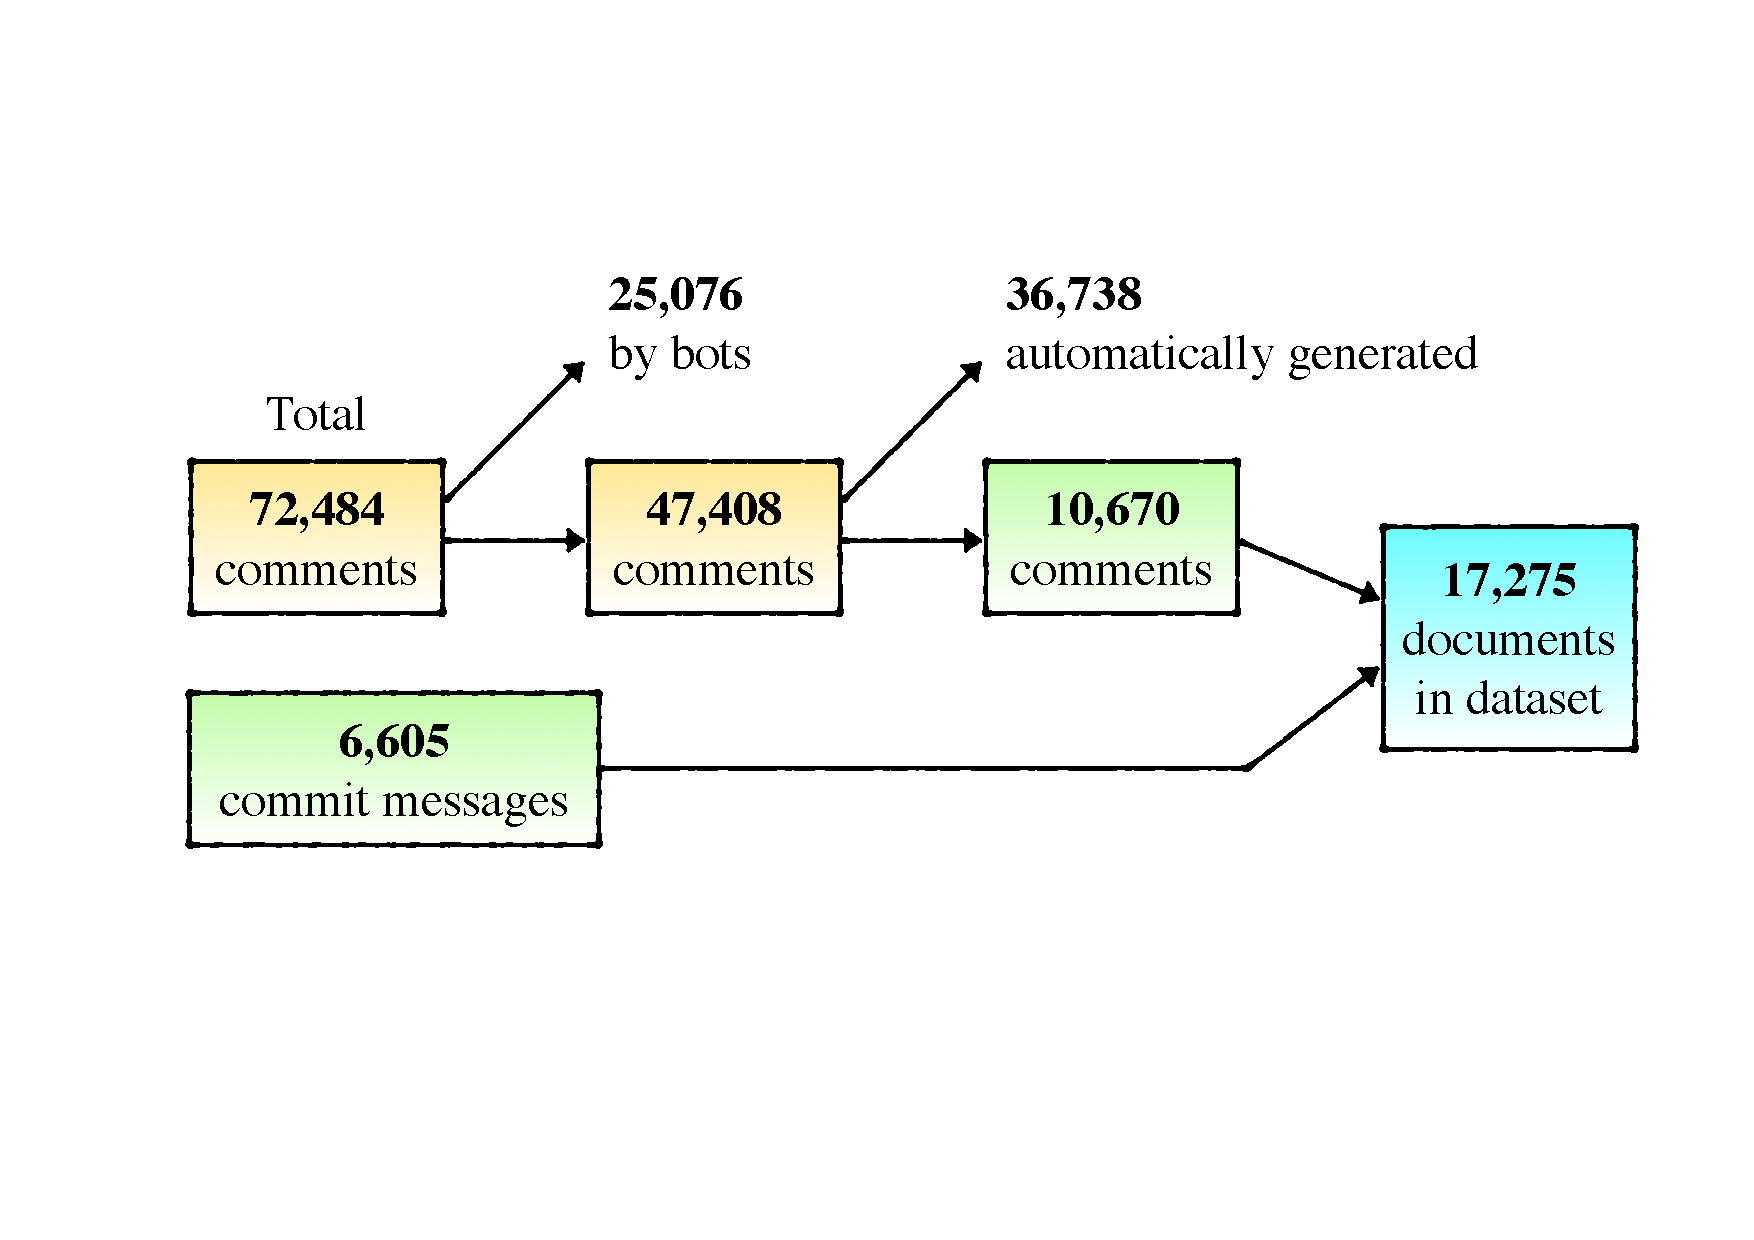
\includegraphics[width=3.2in]{filter}
%\caption{The filtering process.}
%\label{fig:filter}
%\end{figure}
%\subsection{Data Preparation}
%\subsubsection{Data extraction}
%
%6,605 changes and 72,484 comments have been extracted from the raw dataset.
%35\% of the comments are by the system or one of the bots, and are thus discarded.
%
%\subsubsection{Common pattern removal}
%
%By looking for most frequent lines, common patterns were found, such as \emph{`Uploaded patch set 2.'} and \emph{`Change has been successfully cherry-picked to the staging branch as \dots'}.
%
%Removing occurrences of these patterns leaves 77\% of the remaining comments empty.
%This probably means these comments solely contain automatically-generated text, and are thus discarded.
%This leaves us with 10,670 comments and 6,605 commit messages; a total of 17,275 documents.
%
%\subsubsection{Tokenizing}
%
%After the tokenization step, 393,238 tokens are generated in total. They are composed of 20,025 different words.
%This means that each document will be converted into a vector of 20,025 dimensions, each dimension representing a single word.


\begin{ResearchQuestions}
\item[RQ1:] Is semantic similarity a good indicator of MCR comment usefulness?
\end{ResearchQuestions}

\begin{figure}[!t]
\centering
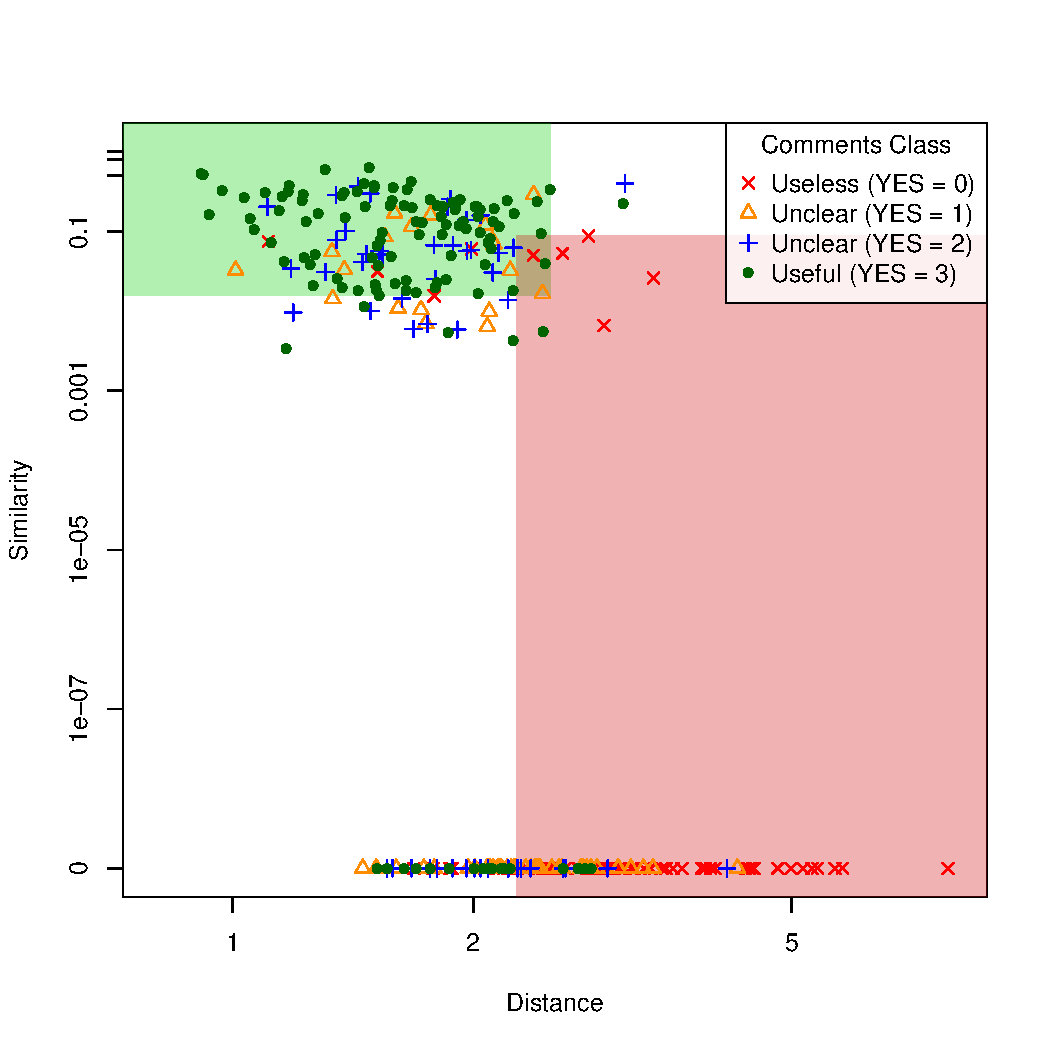
\includegraphics[scale=0.45, trim=0 0 30 50, clip=true]{scatter_log}
\caption{The similarity and distance plot of the training data.
The symbol represents the score, which ranges from 0 to 3.
The green area represents the \emph{useful} classification model and the red area represents the \emph{useless} model.}
\label{fig:scatter}
\end{figure}

To answer this question, we randomly sampled 318 comments from our data set and manually identified usefulness.
Then, we used these comments for both the training and test data set for our approach to determine its effectiveness.
We also determined the effectiveness of our approach using bootstrapping cross validation.

% \dan{What what the effort in person-hours for this?}
% Thai sez:  Average time per comment is 28 seconds.
%            Since we do a lot of other things while training, it gives us a STDEV of 45 seconds.
%            The median, by the way, is just 10 seconds.

% Since our models do not include unclear type of comments, we defined them as negative condition i.e useless comments in case of useful classification (when using $\Theta(c,S_T,D_T)$ model) and useful comments in case of useless classification (when using $\Omega(c,S'_T,D'_T)$ model).
%\dan{I thought we changed this! It would be bad if we didn't. Let me know what the actual situation is here.}
%
% Thai sez:  We did not. Maybe this is just a matter of wording. I believe what the text says is:
%                - For useful classification, we only look for 3 scored comments.
%                - For useless classification, we only look for 0 scored comments.

To determine similarity and dissimilarity thresholds for useful and useless model, we iterated $s_t$ and $d_t$ values from every unique similarity and dissimilarity values in our data set.
%Table \ref{tb:thresholds} shows 5 sets of thresholds that best classify useful and useless comments based on F$_1$ score.
We selected the thresholds that best classify useful and useless comments based on F-measure score and applied models.
The selected models are $\Theta(c,S_T=0.015529,D_T=2.494944)$ for useful comments, and $\Omega(c,S'_T=0.087522,D'_T=2.265679)$ for useless comments.




\textbf{Model Effectiveness Results:} From 318 samples, the comment sets from manual assessment were 85, 60, 51, and 122 for useless set (\texttt{YES} = 0), unclear set (\texttt{YES} = 1 or 2), and useful set (\texttt{YES} = 3), respectively. The precision and Recall of the models were 0.701 and 0.787 for useful model and 0.648 and 0.824 for useless model. 

Figure \ref{fig:scatter} shows the relationship between usefulness class from our classification model and comment sets from manual assessment. 
The green area represents the \emph{useful} classification model and the red area represents the \emph{useless} classification model. The comments drawn in the green area are those satisfied condition of useful model and the comments drawn in the red area are those satisfied condition of useless. While, the comments drawn in the white area are those not satisfied any condition (i.e. \emph{undetermined}). 
The total number of comments from this classification results is described in Table \ref{tb:classify_number}. 



%%Interpret: comments & model%%%%
Corresponding to the precision and recall values, the figure shows that most comments drawn in green area are comments of useful set and very few comments of useless set drawn in this area. Similarly, most comments in the red area are comments of useless set. It also shows that the similarity and dissimilarity values of comments in each set are not different from other comments in the same set. Most of useful set (\texttt{YES} = 3) adhere in the top left of the graph while useless set (\texttt{YES} = 0) adhere in the bottom right of the graph. However, the unclear set still spread out over the graph which we cannot determine relationship between their similarity values.

There is an overlap section as shown in Fig. \ref{fig:scatter}. This is a conflict results between our two models where a comment received true outcome from both classification models.  
This is phenomenon can occur since similarity and dissimilarity values of each group are vague and both  models tend to maximize coverage of classification. However, from the results in Table \ref{tb:classify_number}, only three comments were selected by both models (overlap). This is very small error for our models. Excluding the overlap classification result, we can calculate precision and recall as described in Table \ref{tb:classify_number}. Furthermore, there are 12 useless comments (14\%) and 21 useful comments (17\%) still are undetermined (drawn in white area). These comments were not satisfied our models. This suggests us that other indicators are needed to investigate for usefulness classification.

%From the example comment, it shows that these comments discussed on \TODO{insert topic}, but did not contain any word in common.

\begin{table}[!t]
\centering

\caption{Number of comments classified by our approach against ground truth data}
\begin{tabular}{cccccc}
\hline
Result from & \multicolumn{4}{c}{Results from manual assessment}  & \multirow{3}{*}{Precision}\\ \cline{2-5}
Classification &  Useless  & Unclear  & Unclear & Useful \\
Models&  (\texttt{YES}=0) & (\texttt{YES}=1) & (\texttt{YES}=2) & (\texttt{YES}=3) \\
\hline \hline
Useful & 3 & 12 & 24 & 95 & 0.709\\
Useless & 69 & 23 & 7 & 6 &  0.657\\
Overlap & 1 & 1 & 0 & 1 & - \\
Undetermined & 12 & 24 & 20 & 20 & - \\
\hline
Recall & 0.812 & - & - & 0.778\\ \hline 
\end{tabular}
\label{tb:classify_number}
\end{table}


%\begin{table*}[!t]
%\caption{An accuracy of similarity and dissimilarity thresholds for useful and useless comment classifications}
%\small
%\centering
%\def\arraystretch{1.2}
%\begin{tabular}{ccccccc}
%\hline
%Prediction Models  & Rank & $s_t$ & $d_t$ & F-measure & Precision & Recall \\ \hline \hline
%\multirow{5}{*}{\textbf{useful}: $\Theta(c,S_T=s_t,D_T=d_t)$}
%& 1 & 0.015529 & 2.494944 & 0.741 & 0.701 & 0.787 \\ \cline{2-7}
%& 2 & 0.015529 & 3.077129 & 0.740 & 0.693 & 0.795 \\ \cline{2-7}
%& 3 & 0.016713 & 2.494944 & 0.739 & 0.704 & 0.779 \\ \cline{2-7}
%& 4 & 0.015411 & 2.494944 & 0.738 & 0.696 & 0.787 \\ \cline{2-7}
%& 5 & 0.015411 & 3.077129 & 0.738 & 0.688 & 0.795
%% \\ \cline{2-7}
%% & \multicolumn{3}{r}{Average} &  1.00 & 1.00 & 1.00 \\ \cline{2-7}
%%& \multicolumn{3}{r}{Min-Max} &   1.00 - 1.00 & 1.00 - 1.00  & 1.00 - 1.00
%\\ \hline \hline
%\multirow{5}{*}{\textbf{useless}: $\Omega(c,S'_T=s_t,D'_T=d_t)$}
%& 1 & 0.087522 & 2.265679 & 0.725 & 0.648 & 0.824 \\ \cline{2-7}
%& 2 & 0.087522 & 2.250422 & 0.722 & 0.642 & 0.824 \\ \cline{2-7}
%& 3 & 0.087522 & 2.324771 & 0.720 & 0.663 & 0.788 \\ \cline{2-7}
%& 4 & 0.052856 & 2.265679 & 0.719 & 0.645 & 0.812 \\ \cline{2-7}
%& 5 & 0.087522 & 2.249675 & 0.718 & 0.636 & 0.824
%% \\ \cline{2-7}
%%& \multicolumn{3}{r}{Average} &  1.00 & 1.00 & 1.00 \\ \cline{2-7}
%%& \multicolumn{3}{r}{Min-Max} &   1.00 - 1.00 & 1.00 - 1.00  & 1.00 - 1.00
%\\ \hline
%\end{tabular}
%\label{tb:thresholds}
%\end{table*}

\begin{table*}[!t]
\caption{Results from bootstrapping cross validation of our classification models against random models}
\small
\centering
\def\arraystretch{1.2}
\begin{tabular}{cccc|cc|cc|cc}
\hline
\multicolumn{2}{c}{Classifcation}   & \multicolumn{2}{c|}{Precision} & \multicolumn{2}{c|}{Recall} & \multicolumn{2}{c|}{F-measure} & \multicolumn{2}{c}{Accuracy} \\ \cline{3-10}
\multicolumn{2}{c}{Models} & Avg. & STD. & Avg. & STD. & Avg. & STD. & Avg. & STD. \\ \hline \hline
\multirow{2}{*}{Useful} & $\Theta(c,S_T,D_T)$    &  0.654 & 0.116 &  0.759 & 0.123 & 0.693 & 0.089 & 0.752 & 0.067 \\ \cline{2-10}
& Random     &  0.421 & 0.114 &  0.376 & 0.116 & 0.496 & 0.144 & 0.496 & 0.089 \\ \hline
\multirow{2}{*}{Useless}  & $\Omega(c,S'_T,D'_T)$  &  0.636 & 0.144 &  0.755 & 0.148 & 0.681 & 0.118 & 0.815 & 0.064 \\ \cline{2-10}
& Random    &  0.336 & 0.131 &  0.269 & 0.115 & 0.478 & 0.182 & 0.500 & 0.089 \\
\hline
\end{tabular}
\label{tb:xvalidate}
\end{table*}


\textbf{Validation:}
We validated our approach using bootstrapping cross validation.
We randomly selected 90\% of 318 comments for training set and determine thresholds.
The constructed model is then applied on the remaining 10\% comments as the validation set.
The precision, recall and F-measure scores are measured and recorded.
This validation was repeated 300 times to give an average performance of our models.
For a baseline, we also determined the performance of the random classifier using the same methods.

Table \ref{tb:xvalidate} describes the performance of useful and useless classification models including an average and standard deviation of precision, recall, and F-measure.
The results show that both of our models can achieve 60\% of precision and 75\% of recall, approximately.
In addition, our models also achieved higher results than the random models twice for both precision and recall.


%\begin{table*}[!t]
%\caption{An accuracy of similarity and dissimilarity thresholds for useful and useless comment classifications}
%\small
%\centering
%\def\arraystretch{1.2}
%\begin{tabular}{ccccccc}
%\hline
%Prediction Models & $s_t$ & $d_t$ & F-measure & Precision & Recall \\ \hline \hline
%$\Theta(c,S_T=s_t,D_T=d_t)$   & 0.015529 & 2.494944 & 0.741 & 0.701 & 0.787 \\ \hline
%$\Omega(c,S'_T=s_t,D'_T=d_t)$ & 0.087522 & 2.265679 & 0.725 & 0.648 & 0.824 \\ \hline
%\end{tabular}
%\label{tb:thresholds}
%\end{table*}




According to the results, we can answer RQ1 that \emph{using semantic similarity values as indicators, our approach successfully classify comment usefulness with precision of 0.6 and recall of 0.7 approximately and this is better than random model as twice.}

%After we performed cross validation, we obtained the following result:
%for positive and negative classifications,
%we obtained an average F$_1$ score of 0.693 and 0.681,
%wit
